%%%%%%%%%%%%%%%%%%%%%%%%%%%%%%%%%%%%%%%%%%%%%%%%%%%%%%%%%%%%%%%%%%%%%%%%%%%%%%
%
% Section file included in main project file using \input{}
%
% Assumes that LaTeX2e macros and packages defined in cg_comp.sty are
%   available
%
%%%%%%%%%%%%%%%%%%%%%%%%%%%%%%%%%%%%%%%%%%%%%%%%%%%%%%%%%%%%%%%%%%%%%%%%%%%%%%

 \section{Tempering the Classical Guitar\label{app:temp}}
 
 \begin{quote}
 Temperament: A compromise between the acoustic purity of theoretically exact intervals, and the harmonic discrepancies arising from their practical employment. --- Dr.\ Theo.\ Baker~\cite{ref:baker1895dmt}
 \end{quote}

Shown in \fig{shift_alhambra8p_ej45_fact_temp}, the factory guitar tuned to 12-TET shows the third string having the greatest error in tuning across the fretboard. Tuning the factory guitar to 12-TET exacts a perfect-fifth in the third string while playing a C major chord in first position. This results in the third string being too sharp (+7 cents) for the other common chords of E major (G\#), A major and D major (A). A way to reduce this error is by lowering the pitch of third string 7 cents below 12-TET with an electronic tuner. Another more comprehensive system is to tune all the strings harmonically to the fifth string, which lowers the third string by 7 cents as well as tempering the remaining strings.

In this particular case, the ``Harmonic Tuning Method'' can be followed using these steps:
 \begin{enumerate}
  \item Begin by tuning the fifth string to A$_2 = 110$~Hz, resulting in a fifth-fret harmonic of A$_4 = 440$~Hz. (This can also be tuned by ear from a A$_4$ tuning fork).
  \item Tune that harmonic to the seventh fret harmonic of the fourth string, which is also A$_4 = 440$~Hz.
  \item From there the seventh fret harmonic on the fifth string (E=329.6) can tune the remaining fretted strings: the ninth fret on the third string, the fifth fret on the second string, and the open first string. \red{Matt, isn't the seventh fret harmonic on the fifth string 330~Hz? I though that's what we decided after we patched up my ancient spreadsheet. I know that it's a tiny difference, though.}
  \end{enumerate}

 \red{I'll find a way to prettify this.}
 ( * = Harmonic)

A*5  = D*7 (A=440)
A*7 = E*5 (E=329.6)
A*7 = G9 (E)
A*7 = B5 (E)
A*7 = E0 (E)


 \begin{figure}
  \centering
  \begin{subfigure}[b]{0.45\textwidth}
   \centering
   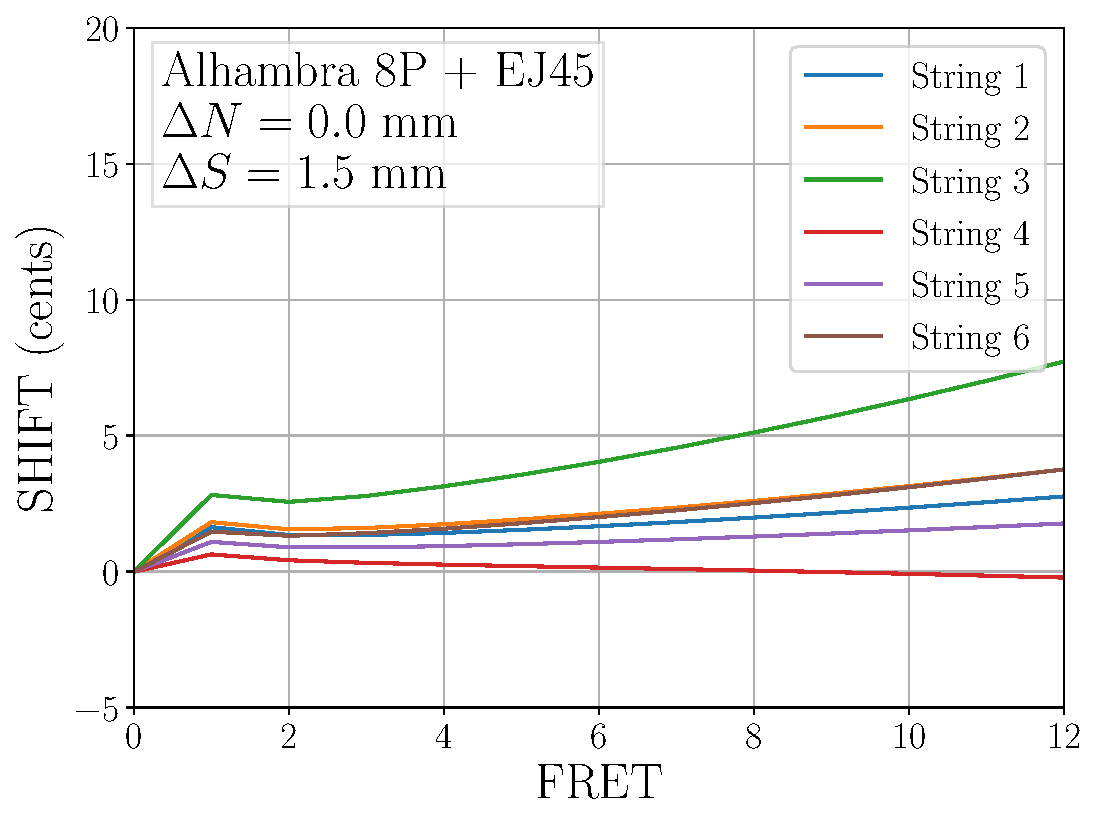
\includegraphics[width=3.25in]{figures/shift_alhambra8p_ej45_factory}
   \caption{Factory guitar --- 12-TET tuned}
   \label{fig:shift_alhambra8p_ej45_fact_temp}
  \end{subfigure}
  \hspace{0.25in}
  \begin{subfigure}[b]{0.45\textwidth}
   \centering
   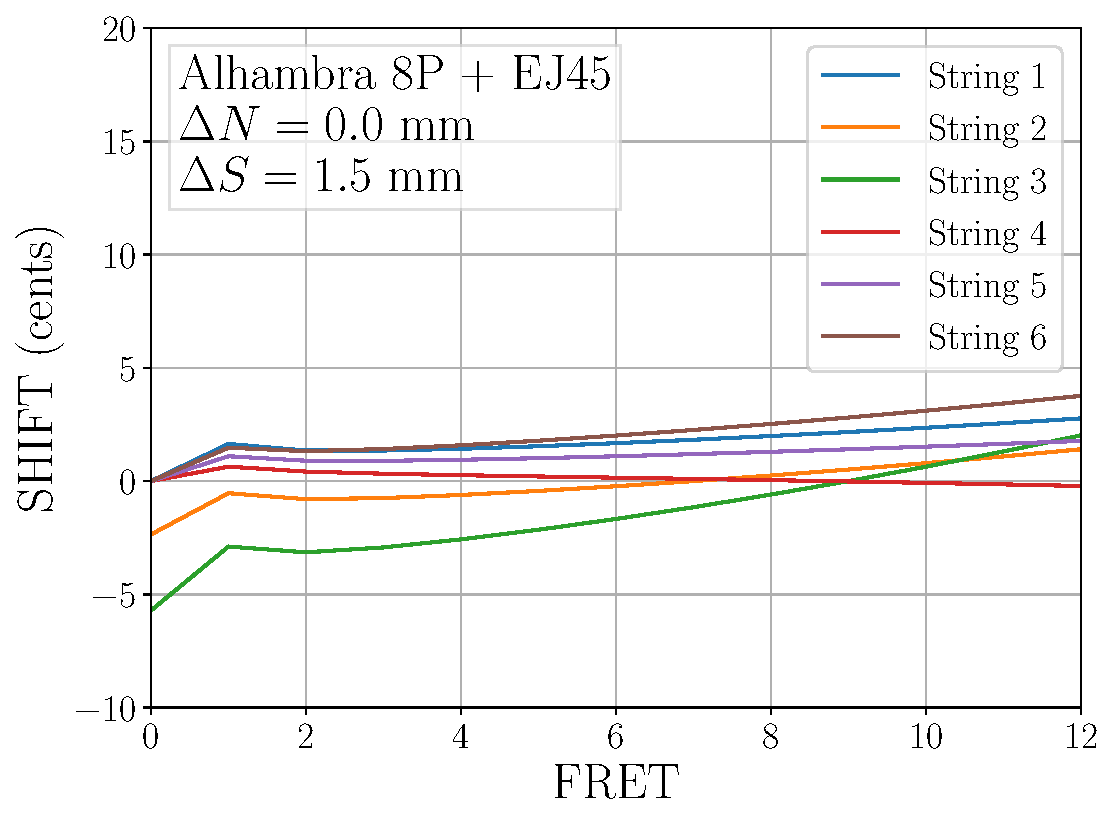
\includegraphics[width=3.25in]{figures/shift_alhambra8p_ej45_harmonic}
   \caption{Factory guitar --- harmonically tuned}
   \label{fig:shift_alhambra8p_ej45_harmonic}
  \end{subfigure}
  \caption{\label{fig:compensation_alhambra8p_ej45_temp} Frequency shift (in cents) for an Alhambra 8P guitar with D'Addario Pro-Arte Nylon Classical Guitar Strings -- Normal Tension (EJ45). Here we compare the factory guitar tuned to 12-TET with the same guitar harmonically tuned.}
 \end{figure}

Next: E and C chords.